
\documentclass[xcolor=usenames]{beamer} % aspectratio=169

\usepackage{fancyvrb}
\usepackage{graphics}
\usepackage[utf8]{inputenc}
\usepackage{amsmath}
%\usepackage{lmodern}
\usepackage{amssymb}
\usepackage{MnSymbol}
\usepackage[normalem]{ulem} % for strikeout
%\usepackage{verbatim} % TODO uncomment later
%\usepackage{tikz}
\usepackage{textcomp} % copy-pastable chars
\usepackage{hyperref}
\hypersetup{
	pdfauthor={Nicholas Dahm (Dr. Nick)},
	pdfsubject={Computer Vision},
	pdftitle={Hacking the Visual World with OpenCV},
	pdfkeywords={OpenCV, Python}
}

\mode<presentation>
{
	%\usetheme{Warsaw}
	\usetheme{Madrid}
	%\usetheme{Torino}
	\setbeamercovered{transparent}

	\usefonttheme{serif}

	% COLOURS
	%\usecolortheme{spruce}
	%\setbeamercolor{local structure}{fg=??} % Make everything inherit theme colours

	\usecolortheme{beaver} % needs different bullet colours
	\setbeamercolor{local structure}{fg=darkred} % Make everything inherit theme colours

	%\setbeamercolor{item projected}{bg=darkred}
	%\setbeamertemplate{enumerate items}[default]
	%\setbeamercolor{block title}{fg=darkred}

	\setbeamertemplate{navigation symbols}{}


	\setbeamertemplate{itemize item}{$\blacktriangleright$}
	%\setbeamertemplate{itemize subitem}{$\triangleright$}
	\setbeamertemplate{itemize subitem}{-}
}

\AtBeginSection[]
{
	\begin{frame}<beamer>{}
		\tableofcontents[currentsection,currentsubsection]
	\end{frame}
}

\AtBeginSubsection[]
{
	\begin{frame}<beamer>{}
		\tableofcontents[currentsection,currentsubsection]
	\end{frame}
}


\newcommand{\bi}{\begin{itemize}}
\newcommand{\ei}{\end{itemize}}

\newcommand{\be}{\begin{enumerate}}
\newcommand{\ee}{\end{enumerate}}

\newcommand{\degrees}{^\circ}

\newcommand{\bc}[1][0.5]{\begin{column}{#1\textwidth}}
\newcommand{\ec}{\end{column}}

\newcommand{\bci}[1][0.5]{\begin{column}{#1\textwidth} \begin{itemize}}
\newcommand{\eci}{\end{itemize}\end{column}}

% This allows putting images arbitrarily on slides
\def\Put(#1,#2)#3{\leavevmode\makebox(0,0){\put(#1,#2){#3}}}


\usepackage{listings}
\usepackage{color}

\definecolor{dkgreen}{rgb}{0,0.6,0}
\definecolor{gray}{rgb}{0.5,0.5,0.5}
\definecolor{mauve}{rgb}{0.58,0,0.82}

\lstset{frame=tb,
	language=python,
	aboveskip=3mm,
	belowskip=3mm,
	showstringspaces=false,
	columns=flexible,
	basicstyle={\small\ttfamily},
	numbers=none,
	numberstyle=\tiny\color{gray},
	keywordstyle=\color{blue},
	commentstyle=\color{dkgreen},
	stringstyle=\color{mauve},
	breaklines=true,
	breakatwhitespace=true,
	tabsize=4,
	upquote=true
}





\title[Hacking the Visual World]{Hacking the Visual World with OpenCV}
\subtitle{Computer Vision in Python}
\date{January 25, 2017}
\author[Dr. Nick]{Nicholas Dahm / Dr. Nick / Aussie Nick}
\institute[TrademarkVision]{
	\Large
	TrademarkVision\\\vspace{4mm}
	\normalsize
	\textit{Code \& slides available at:}\\\url{https://github.com/das-intensity/presidential}
}
\subject{Computer Vision} % PDF properties only


%%% IMAGE SOURCES IN THIS PRESENTATION %%%
% NOTE: Most images in this presentation were listed as available for non-commercial reuse by google or via public domain image sites. Please directly confirm the copyright status of them before reuse.
% EXCEPTIONS:
%-The tmv-results.png image was taken via screenshot of the trademark.vision system. The logos within it are of course copyright protected, and as such, this image should not be reused elsewhere.
%-The tmv-logo.png is copyright protected, but permission was obtained to include it in this presentation. Reuse prohibited.

% face-tracking.png <- https://upload.wikimedia.org/wikipedia/commons/4/4e/Visage_Technologies_Face_Tracking_and_Analysis.png
% nasa-robot.jpg <- https://c3.staticflickr.com/5/4083/5161877250_7bc25c9e19_b.jpg
% fpv-hud.png <- https://upload.wikimedia.org/wikipedia/commons/d/d2/FPV_OSD.png
% camera-transformer.jpg <- https://c1.staticflickr.com/2/1062/835831228_7e2bc6a207.jpg
% hyperspectral.png <- https://upload.wikimedia.org/wikipedia/en/7/77/Specim_aisaowl_outdoor.png
% python.svg <- https://pixabay.com/get/ea34b30a2ef51c3e955e4600e1444e9efe76e6dd1cb2134290f5c1/snake-312561.svg?attachment
% opencv.svg <- https://upload.wikimedia.org/wikipedia/commons/3/32/OpenCV_Logo_with_text_svg_version.svg?download
% numpy.png <- https://upload.wikimedia.org/wikipedia/en/1/1b/NumPy_logo.png?download
% mag.svg <- https://upload.wikimedia.org/wikipedia/commons/3/3a/Magnifying_glass_01.svg
% hsv.png <- https://upload.wikimedia.org/wikipedia/commons/thumb/0/0d/HSV_color_solid_cylinder_alpha_lowgamma.png/320px-HSV_color_solid_cylinder_alpha_lowgamma.png
% The *-hog.jpg images were created with the hog visualisation tool here: http://www.cs.cornell.edu/courses/cs4670/2012fa/projects/p5/index.html


\begin{document}
%\part<presentation>{Front}
\begin{frame}
	\titlepage
\end{frame}


\begin{frame}
	\tableofcontents
\end{frame}


\section{What is Computer Vision?}
\begin{frame}{What is Computer Vision?}
	\Put(0,100){\includegraphics[height=35mm]{images/fpv-hud}}% TOP LEFT
	\Put(0,-240){\includegraphics[height=35mm]{images/hyperspectral}}% BOTTOM LEFT
	%
	\Put(180,150){\includegraphics[height=35mm]{images/nasa-robot}}% TOP RIGHT
	\Put(240,-240){\includegraphics[height=35mm]{images/face-tracking}}% BOTTOM RIGHT
	%
	\Put(100,0){\includegraphics[height=35mm]{images/camera-transformer}}% MIDDLE
\end{frame}


\begin{frame}{What is the data?}
	\Put(0,100){\includegraphics[height=30mm]{images/mantis-shrimp}}%
	\Put(210,20){\includegraphics[height=30mm]{images/mantis-shrimp-blue}}%
	\Put(160,-150){\includegraphics[height=30mm]{images/mantis-shrimp-green}}%
	\Put(110,-240){\includegraphics[height=30mm]{images/mantis-shrimp-red}}%
\end{frame}


\begin{frame}{How to Computer Vision a thing?}
	\bi
		\item \textbf{Object detection} - where are the faces in this image?
		\item \textbf{Object recognition} - is that face John Smith?
		\item \textbf{Object classification} - which animal is this?
		\item \textbf{Image matching} - how similar are these images?
		\item \textbf{Image retrieval} - what images look similar to this?
		\item \textbf{Object tracking} - watch where that car goes
		\item \textbf{Scene reconstruction} - create a 3D model from this video
		\item \textbf{Image restoration} - remove the wrinkle from this scanned photo
	\ei
\end{frame}


\begin{frame}{TrademarkVision - image retrieval}
	%\Put(0,100){\includegraphics[height=35mm]{images/tmv-results}}% TOP LEFT
	\centering
	\includegraphics[height=0.8\textheight]{images/tmv-results}
\end{frame}


\begin{frame}{Image features - HOG}
	\Put(0,100){\includegraphics[height=35mm]{images/tmv-logo}}% TOP LEFT
	\Put(160,100){\Huge $\rightarrow$}% TOP LEFT
	\Put(230,100){\includegraphics[height=33mm]{images/tmv-logo-hog}}% TOP RIGHT
	%
	\Put(20,-240){\includegraphics[height=35mm]{images/mag}}% BOTTOM LEFT
	\Put(160,-140){\Huge $\rightarrow$}% TOP LEFT
	\Put(240,-240){\includegraphics[height=35mm]{images/mag-hog}}% BOTTOM RIGHT
	%Talk about tracking, segmentation, image matching. Give some examples, e.g. what we do at TMV
\end{frame}


\begin{frame}{Comparing image features}
	\Put(0,100){\includegraphics[height=35mm]{images/tmv-logo-hog}}% TOP LEFT
	\Put(140,100){\Huge $\rightarrow$}% TOP LEFT
	\Put(180,100){$(0.20, 0.04, 0.07, 0.12, \ldots, 0.11)$}% TOP RIGHT
	%
	\Put(150,0){Diff $= (0.07, 0.14, 0.06, 0.08, \ldots, 0.01)$}%
	\Put(157,-40){$L_1 = 0.52$}%
	%
	\Put(10,-240){\includegraphics[height=35mm]{images/mag-hog}}% BOTTOM LEFT
	\Put(140,-140){\Huge $\rightarrow$}% TOP LEFT
	\Put(180,-140){$(0.13, 0.18, 0.01, 0.04, \ldots, 0.12)$}% TOP RIGHT
	%Talk about tracking, segmentation, image matching. Give some examples, e.g. what we do at TMV
\end{frame}


\begin{frame}{Computer Vision in Python}
	What Computer Vision tools are available for us in Python?
	\bi
		\item OpenCV
		\bi
			\item Large library of computer vision functions
			\item Many algorithms for all types of tasks
			\item Python wrapper for underlying C++ library
			\item Stores images as NumPy arrays for easy manipulation
		\ei
		\item NumPy
		\bi
			\item Extensive matrix manipulation library
			\item Incredibly fast when using matrix operations
		\ei
		\item PIL
		\bi
			\item Python Imaging Library (or newer Pillow fork)
			\item Various image operations, including some not in OpenCV
			\item Quick translations to/from OpenCV's NumPy format
		\ei
	\ei
\end{frame}


\section{Example: The Presidential Look}
\begin{frame}{Prerequisites}
	\bi
		\item Python (2.7 recommended)
		\item OpenCV (3 recommended)
		\item NumPy
		\item PIL (optional)
	\ei
	\Put(10,-220){\includegraphics[height=40mm]{images/python}}%
	\Put(170,50){\includegraphics[height=50mm]{images/opencv}}%
	%\Put(180,-200){\fbox{\bf \Huge NumPy}}%
	\Put(180,-220){\includegraphics[height=15mm]{images/numpy}}%
	\vspace{40mm}
\end{frame}


\begin{frame}[fragile]{A Wild Squirrel Appears!}
	\Put(220,-220){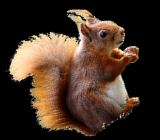
\includegraphics[height=35mm]{images/squirrel}}%
	\vspace{-2mm}
	\begin{lstlisting}
import cv2
import numpy as np

# Download goo.gl/nXaoEf as squirrel.png

sq = cv2.imread('squirrel.png')
print sq.shape # (140, 160, 3)
cv2.imshow('squirrel', sq)

sq_gray = cv2.cvtColor(sq, cv2.COLOR_BGR2GRAY)
print sq_gray.shape # (140, 160)
cv2.imshow('squirrel gray', sq_gray)
cv2.waitKey()
	\end{lstlisting}
	\vspace{-1mm}
	\bi
		\item You used computer vision... it's super effective!
	\ei
\end{frame}


\begin{frame}{OpenCV Squirrel Windows}
	\Put(40,0){\includegraphics[height=45mm]{images/step-squirrels}}%
\end{frame}


% TODO remove this slide?
\begin{frame}[fragile]{PIL~\textless-\textgreater~OpenCV}
	\begin{lstlisting}
from PIL import Image
pilsq = Image.open('squirrel.png')

# PIL -> cv2
sq2 = np.asarray(pilsq)
sq2 = cv2.cvtColor(sq2, cv2.COLOR_RGB2BGR)
# cv2 -> PIL
pilsq2 = cv2.cvtColor(sq2, cv2.COLOR_BGR2RGB)
pilsq2 = Image.fromarray(pilsq2)
	\end{lstlisting}
\end{frame}


\begin{frame}[fragile]{I wanna see myself!}
	\begin{lstlisting}
print 'starting webcam...'
cam = cv2.VideoCapture(0)
ret, frame = cam.read()
assert ret # fails if couldn't read from webcam
print 'webcam res:', frame.shape

while True:
    ret, frame = cam.read()

    cv2.imshow('cam', frame)
    key = cv2.waitKey(1)
    if key != -1:
        break
	\end{lstlisting}
\end{frame}


\begin{frame}{Hi everybody!}
	\Put(90,0){\includegraphics[height=45mm]{images/step-webcam}}%
\end{frame}


\begin{frame}[fragile]{I still want the squirrel though!}
	\begin{lstlisting}
sq_gray_mask = sq_gray > 0
sq_mask = np.array(
		[[[v, v, v] for v in row] for row in sq_gray_mask]
		)

while True:
    ret, frame = cam.read()

    # overlay the squirrel
    np.copyto(
			frame[-sq.shape[0]:, 0:sq.shape[1], :],
			sq,
			where=sq_mask
			)

    cv2.imshow('cam', frame)
	\end{lstlisting}
\end{frame}


\begin{frame}{A ``Squirrel Productions'' film}
	\Put(90,0){\includegraphics[height=45mm]{images/step-squirrel-productions}}%
\end{frame}


\begin{frame}[fragile]{Detecting faces}
	\begin{lstlisting}
cas = cv2.CascadeClassifier(
	'/usr/share/opencv/haarcascades/'
	+ 'haarcascade_frontalface_default.xml'
	)
	\end{lstlisting}
	\begin{lstlisting}
	### inside while loop, after cam.read() ###
    frame_gray = cv2.cvtColor(frame, cv2.COLOR_BGR2GRAY)
    faces = cas.detectMultiScale(
            frame_gray,
            scaleFactor=1.1,
            minNeighbors=5,
            minSize=(30, 30),
            flags = cv2.CASCADE_SCALE_IMAGE
            # OpenCV 2.4 -> cv2.cv.CV_HAAR_SCALE_IMAGE
            )
	# faces is list of (x, y, width, height)
	\end{lstlisting}
\end{frame}


\begin{frame}[fragile]{Drawing faces}
	\begin{lstlisting}
    for (x, y, w, h) in faces:
        cv2.rectangle(frame, (x, y), (x+w, y+h), (0, 255, 0), 2)

		# Make the box a bit bigger (see why later)
		#- first save originals
        x0 = x; y0 = y; w0 = w; h0 = h

        h += int(h * 0.3)
        x -= int(w * 0.1)
        w += int(w * 0.2)
        if y < 0 or y+h > frame.shape[0]: continue
        if x < 0 or x+w > frame.shape[1]: continue

        cv2.rectangle(frame, (x, y), (x+w, y+h), (0, 255, 255), 2)
	\end{lstlisting}
\end{frame}


\begin{frame}{FaceBox.. the latest social media craze}
	\Put(90,0){\includegraphics[height=45mm]{images/step-face-detection}}%
\end{frame}


\begin{frame}[fragile]{Find the non-presidential skin...}
	\begin{lstlisting}
		### inside faces loop ###
        # Find the skin pixels
        frame_hsv = cv2.cvtColor(frame, cv2.COLOR_BGR2HSV)
        face_hsv = frame_hsv[y:y+h, x:x+w, :]

        hsv_min = np.array([0, 0, 40])
        hsv_max = np.array([200, 120, 220])
        face_inrange = cv2.inRange(face_hsv, hsv_min, hsv_max)
        face_inrange = np.array([[[v, v, v] for v in row] for row in face_inrange], dtype=bool)
        #print 'face_inrange: %s - %s' % (face_inrange.shape, face_inrange.dtype)
	\end{lstlisting}
\end{frame}

\begin{frame}[fragile]{Upgrade it to a more presidential colour}
	\begin{lstlisting}
		### inside faces loop ###
		# Set a more presidential color
        pres_skin = [0.2, 0.65, 1.7]
        face_bgr = frame[y:y+h, x:x+w, :] * pres_skin
        face_bgr = np.minimum(face_bgr, 255)
        face_bgr = np.array(face_bgr, dtype='uint8')
        #print 'face_bgr: %s - %s' % (face_bgr.shape, face_bgr.dtype)
        np.copyto(frame[y:y+h, x:x+w, :], face_bgr, where=face_inrange)
	\end{lstlisting}
\end{frame}


\begin{frame}{Orange is the presidential colour}
	\Put(90,0){\includegraphics[height=45mm]{images/step-presidential-skin}}%
\end{frame}


\begin{frame}[fragile]{Let get some presidential hair!}
	\begin{lstlisting}
		### inside faces loop ###
        # Obtain some presidential hair
        hair = sq[30:,0:70]
        hair = np.rot90(hair, 3)
        hair_mask = sq_mask[30:,0:70]
        hair_mask = np.rot90(hair_mask, 3)

        hair_scale = w0 / float(hair.shape[1])

        hair = cv2.resize(hair, None, fx=hair_scale, fy=hair_scale)
	\end{lstlisting}
\end{frame}

\begin{frame}[fragile]{Wear the presidential hair!}
	\begin{lstlisting}
		### inside faces loop ###
		# Wear the presidential hair!
        hair_mask = np.array(hair_mask, dtype='uint8')
        hair_mask = cv2.resize(hair_mask, None, fx=hair_scale, fy=hair_scale)
        hair_mask = np.array(hair_mask, dtype=bool)

        hair = np.array(np.minimum((hair * 0.7) + 100, 255), dtype='uint8') # Optional

        if y0 - hair.shape[0] < 0: continue
        np.copyto(frame[y0-hair.shape[0]:y0, x0:x0+hair.shape[1], :], hair, where=hair_mask)
	\end{lstlisting}
\end{frame}


\begin{frame}{The most presidential look, period!}
	\Put(90,0){\includegraphics[height=45mm]{images/step-presidential-hair}}%
\end{frame}

\begin{frame}{Thanks for listening!}
	\centering
	Never let the visual reality get in your way again! \\
	\includegraphics[height=45mm]{images/computer-eye} \\\vspace{4mm}
	\href{https://trademark.vision}{trademark.vision}\\
	\href{github.com/das-intensity}{github.com/das-intensity}\\
	\href{linkedin.com/in/nicholasdahm}{linkedin.com/in/nicholasdahm}\\
	\href{meetup.com/members/195619601}{meetup.com/members/195619601}
\end{frame}

\end{document}

